% Provenance (never printed): enseignement scientifique premiere (2019),
% "La Terre, un astre singulier" (the place of the Earth) and the old seconde
% SVT "La planete Terre, une planete habitable" (conditions for liquid water,
% the habitable zone); see sources/book2/PROVENANCE.md. Every temperature,
% phase boundary and habitable-zone limit is computed in
% figdata/grade-10/planet_temperatures.py.
\chapter{Een bewoonbare planeet}\label{ch:g10:habitable-planet}

Drie rotsplaneten draaien naast elkaar om de Zon. Aan het oppervlak van Venus
is de lucht zo dicht dat ze tweeënnegentig keer harder drukt dan op Aarde, en
zo heet --- meer dan \qty{460}{\degreeCelsius} --- dat lood er zou smelten.
Op Mars drukt de ijle lucht nog geen honderdste zo hard als de onze, en ligt
de gemiddelde temperatuur ver onder het vriespunt. Daartussen heeft de Aarde
oceanen, regen en leven. De drie planeten zijn ontstaan uit dezelfde schijf van
gas en stof rond de jonge Zon, uit grotendeels hetzelfde gesteente. Waarom
dan zo'n verschillend lot? Dit hoofdstuk bekijkt wat de temperatuur van een
planeet bepaalt, waardoor ze een atmosfeer kan vasthouden, onder welke
voorwaarden water vloeibaar kan zijn, en waar, rond de Zon en rond andere
sterren, zulke voorwaarden te vinden zijn.
% ledger: nasa:venus-atm, nasa:mars-atm, planet:Venus.Tmean

\begin{omfigure}
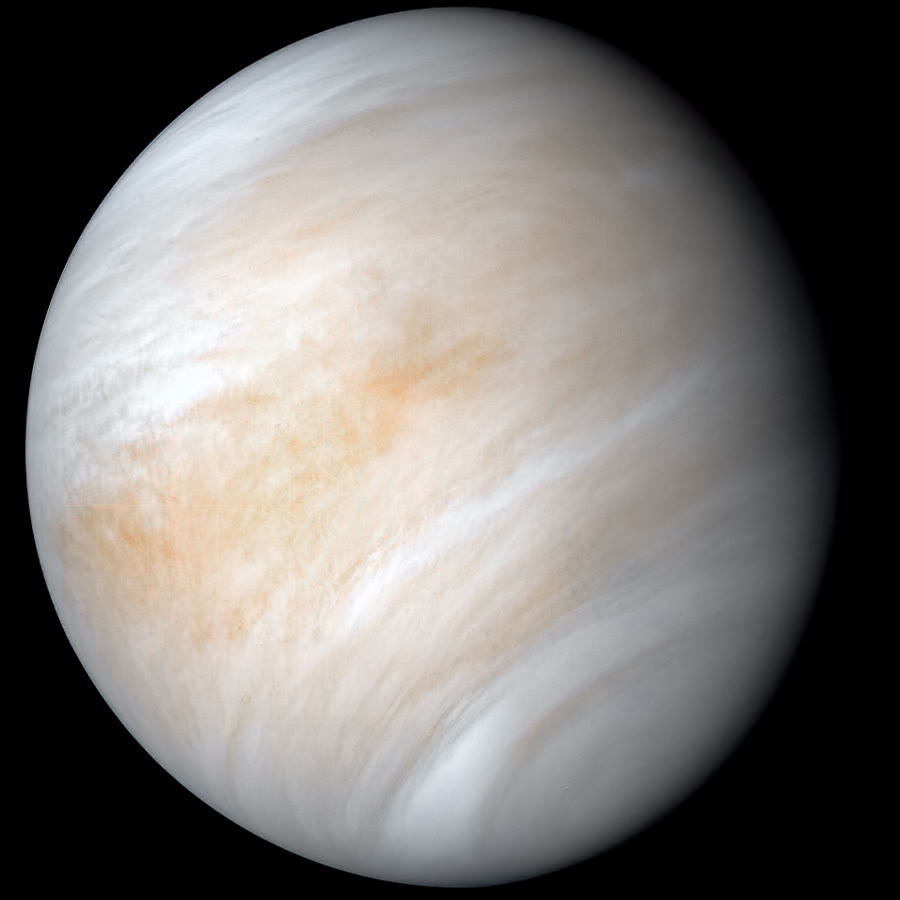
\includegraphics[width=0.38\linewidth]{images/book2/g10-nasa-venus-mariner10.jpg}

{\small Venus, gezien door de ruimtesonde Mariner~10 in 1974, in kleuren die
dicht bij wat het oog zou zien liggen: een planeet die helemaal in wolken is
gehuld. Beeld: NASA/JPL-Caltech (publiek domein).}
\end{omfigure}

\begin{recall}
De Zon is een ster; om haar heen draaien de vier rotsplaneten Mercurius, Venus,
de Aarde en Mars, en daarna de vier reuzenplaneten, in bijna cirkelvormige
banen (de natuurkundeboeken en Boek 1). Elk lichaam straalt energie uit als
licht, des te meer naarmate zijn temperatuur stijgt, bij de temperaturen van
planeten vooral als infrarood licht (de natuurkundeboeken). Broeikasgassen ---
waterdamp, koolstofdioxide, methaan --- absorberen een deel van het infrarood
dat een oppervlak uitzendt en houden het warmer (de scheikundeboeken). Water
bestaat als ijs, vloeibaar water en waterdamp; druk is een kracht per
oppervlakte-eenheid, gemeten in pascal (de natuurkundeboeken).
\end{recall}

\section{De temperatuur die de ster oplegt}

De Zon zendt haar licht gelijkmatig in alle richtingen uit. Op een afstand $d$
is haar vermogen $L$ (haar \emph{lichtkracht}) verdeeld over een bol met oppervlakte $4\pi d^2$.

\begin{proposition}[De omgekeerd-kwadratenwet van het zonlicht]\label{prop:g10:habitable-planet:inverse-square}
Het vermogen dat per vierkante meter loodrecht op de zonnestralen wordt
ontvangen, de \emph{bestralingssterkte} van de Zon, is op een afstand $d$ van de Zon
\[
  S = \frac{L}{4\pi d^2}.
\]
Op de afstand van de Aarde, \qty{1}{au}, is $S_0 = \qty{1361}{W/m^2}$; op een
afstand $d$ gemeten in astronomische eenheden is $S = S_0/d^2$.
\end{proposition}

\begin{proof}
In de lege ruimte gaat geen licht verloren, dus het hele vermogen $L$ gaat door
elke bol met de Zon als middelpunt; op een bol met straal $d$ wordt het verdeeld
over $4\pi d^2$ vierkante meter. Verdubbelt $d$, dan wordt de oppervlakte vier
keer zo groot en $S$ vier keer zo klein.
\end{proof}
% ledger: earth:TSI, sun:L, const:au

\begin{omfigure}
\begin{tikzpicture}[font=\small, >={Stealth[length=2mm]}]
  \shade[ball color=yellow!70!orange] (0,0) circle (0.35);
  \node[below=4pt] at (0,-0.35) {Zon};
  \draw[omThm!70, thick] (0,0) -- (3,0.6) (0,0) -- (3,-0.6);
  \draw[omThm!70, thick, dashed] (3,0.6) -- (6,1.2) (3,-0.6) -- (6,-1.2);
  \draw[fill=omDef!25, draw=omDef!80!black] (3,-0.6) rectangle (3.18,0.6);
  \draw[fill=omDef!12, draw=omDef!80!black] (6,-1.2) rectangle (6.18,1.2);
  \draw[omDef!80!black] (6,0) -- (6.18,0) (6.09,-1.2) -- (6.09,1.2);
  \node[anchor=north] at (3.1,-0.7) {$d$};
  \node[anchor=north] at (6.1,-1.3) {$2d$};
  \node[anchor=south east, align=right, font=\footnotesize] at (2.9,0.75) {1 vierkant:\\al het licht};
  \node[anchor=west, align=left, font=\footnotesize] at (6.35,0.6) {4 vierkanten:\\elk een kwart};
  \draw[->, black!60] (0.5,-1.95) -- (6.1,-1.95);
  \node[anchor=north, font=\footnotesize] at (3.3,-2.0) {afstand tot de Zon};
\end{tikzpicture}

{\small Het licht dat op afstand $d$ door één vierkant gaat, is op afstand $2d$
verdeeld over vier even grote vierkanten: de bestralingssterkte neemt af met
het kwadraat van de afstand.}
\end{omfigure}

Een planeet absorbeert het deel van dit licht dat ze niet weerkaatst, en ze
straalt energie uit naar de ruimte als infrarood licht. Absorbeert ze meer dan
ze uitstraalt, dan warmt ze op; warmer straalt ze meer uit; ze komt tot rust
bij de temperatuur waarbij die twee in evenwicht zijn.

\begin{definition}[Evenwichtstemperatuur]\label{def:g10:habitable-planet:equilibrium-temperature}
De \emph{evenwichtstemperatuur}\index{evenwichtstemperatuur} van een
planeet is de temperatuur waarbij een lichaam dat straalt als een perfecte
straler, precies het vermogen naar de ruimte zou uitzenden dat de planeet van
haar ster absorbeert. Het deel van het invallende licht dat de planeet als
geheel weerkaatst, is haar \emph{bondalbedo} $A$.
\end{definition}

\begin{proposition}[De evenwichtstemperatuur berekenen]\label{prop:g10:habitable-planet:teq}
Voor een planeet die de warmte die ze absorbeert over haar hele oppervlak verdeelt, geldt
\[
  T_{\mathrm{eq}} = \left(\frac{S\,(1-A)}{4\sigma}\right)^{1/4},
  \qquad \sigma = \qty{5.67e-8}{W.m^{-2}.K^{-4}}.
\]
Op de afstand van de Aarde en zonder enige weerkaatsing geeft dit
\qty{278.3}{K}; op een afstand $d$ in astronomische eenheden en met albedo $A$
is $T_{\mathrm{eq}} = \qty{278.3}{K} \times (1-A)^{1/4}/\sqrt{d}$.
\end{proposition}

\begin{proof}[Gedeeltelijk bewijs]
De planeet onderschept zonlicht op een schijf met oppervlakte $\pi R^2$ en
absorbeert het vermogen $(1-A)\,S\,\pi R^2$. Ze straalt uit over haar hele
oppervlak, $4\pi R^2$. Een perfecte straler met temperatuur $T$ straalt
$\sigma T^4$ per vierkante meter uit (een wet die in de natuurkundeboeken wordt
bewezen en hier wordt aangenomen). Uit
$4\pi R^2 \sigma T^4 = (1-A)\,S\,\pi R^2$ volgt de formule; de straal valt
weg. Met $S = S_0/d^2$ is de vierdemachtswortel van $1/d^2$ gelijk aan $1/\sqrt d$.
\end{proof}
% ledger: const:sigma, earth:TSI

\begin{example}[De Aarde]\label{ex:g10:habitable-planet:earth}
% ledger: earth:TSI, earth:albedo, earth:Tbb, earth:Tsurf
Met $S_0 = \qty{1361}{W/m^2}$ en $A = 0.294$ is
$T_{\mathrm{eq}} = 278.3 \times 0.706^{1/4} \approx \qty{255}{K}$, dat is
\qty{-18}{\degreeCelsius}. (Het gegevensblad van NASA geeft \qty{254}{K}.) De
gemiddelde temperatuur van het aardoppervlak is \qty{288}{K},
\qty{15}{\degreeCelsius}: het broeikaseffect van de atmosfeer warmt het met
ongeveer \qty{33}{K} op. Zonder dat effect zouden de oceanen bevriezen.
\end{example}

\begin{omfigure}
\begin{tikzpicture}
\begin{axis}[ybar, width=0.86\linewidth, height=5.8cm, ymin=0, ymax=950,
  bar width=10pt, enlarge x limits=0.15, symbolic x coords={Mercury,Venus,Earth,Moon,Mars},
  xtick=data, xticklabels={Mercurius,Venus,Aarde,Maan,Mars}, ylabel={temperatuur (K)}, ymajorgrids, grid style={gray!22},
  legend style={at={(0.97,0.95)}, anchor=north east, font=\footnotesize, draw=black!30},
  nodes near coords, nodes near coords style={font=\scriptsize, rotate=90, anchor=west, /pgf/number format/fixed, /pgf/number format/precision=0},
  tick label style={font=\small}, label style={font=\small}]
\addplot[fill=omDef!45, draw=omDef!80!black] table[x=name, y=Teq_K] {figdata/out/grade-10-planet_temperatures-planets.dat};
\addlegendentry{evenwichtstemperatuur}
\addplot[fill=omThm!55, draw=omThm!80!black] table[x=name, y=Tmean_K] {figdata/out/grade-10-planet_temperatures-planets.dat};
\addlegendentry{gemeten gemiddelde oppervlaktetemperatuur}
\end{axis}
\end{tikzpicture}

{\small Evenwichtstemperaturen, berekend uit de afstand en het bondalbedo van
elk hemellichaam, naast de gemeten gemiddelde temperatuur van hun oppervlak.
Gegevens: planetaire gegevensbladen van NASA.}
\end{omfigure}

\begin{remark}[Het diagram lezen]\label{rem:g10:habitable-planet:reading}
% ledger: nasa:bond-albedos, planet:Mercury.Tmean, planet:Venus.Tmean, planet:Moon.Tmean, planet:Mars.Tmean, planet:Moon.day, nasa:moon-temps
Bij Mercurius en Mars, die bijna geen of maar een heel ijle atmosfeer hebben,
ligt het gemeten gemiddelde dicht bij de \omterm{def:g10:habitable-planet:equilibrium-temperature}{evenwichtstemperatuur}. Bij de Maan
ligt het gemiddelde eronder: haar dagen en nachten duren elk ongeveer twee
weken, en haar oppervlak schommelt van ongeveer \qty{95}{K} tot \qty{390}{K},
wat de eenvoudige formule, bedoeld voor een planeet die haar warmte gelijkmatig
verdeelt, niet beschrijft. Venus is het opvallende geval: met een bondalbedo
van 0.77 --- haar wolken weerkaatsen het grootste deel van het zonlicht --- is
haar \omterm{def:g10:habitable-planet:equilibrium-temperature}{evenwichtstemperatuur} lager dan die van de Aarde, en toch is haar
oppervlak meer dan \qty{500}{K} heter: het broeikaseffect van haar dikke
atmosfeer van koolstofdioxide.
\end{remark}

\section{Een atmosfeer vasthouden}

Een gas bestaat uit moleculen die voortdurend bewegen, des te sneller naarmate
het gas heter is. Een molecuul bovenin een atmosfeer dat sneller omhoog beweegt
dan de ontsnappingssnelheid van de planeet --- de snelheid die nodig is om haar
zwaartekracht voorgoed te verlaten (de natuurkundeboeken) --- gaat verloren in
de ruimte. In miljarden jaren verliest een kleine planeet met een zwakke
zwaartekracht haar lucht; een grote houdt ze vast.

\begin{center}
\small
% ledger: planet:Mercury.vesc, planet:Venus.vesc, planet:Earth.vesc, planet:Moon.vesc, planet:Mars.vesc, planet:Mercury.psurf, planet:Venus.psurf, planet:Earth.psurf, planet:Moon.psurf, nasa:mars-atm
\begin{tabular}{lccc}
\hline
hemellichaam & ontsnappingssnelheid (\unit{km/s}) & druk aan het oppervlak (bar) & atmosfeer \\
\hline
Maan & 2.4 & 0 & geen \\
Mercurius & 4.3 & 0 & geen \\
Mars & 5.0 & 0.006 & ijl, koolstofdioxide \\
Venus & 10.4 & 92 & dik, koolstofdioxide \\
Aarde & 11.2 & 1 & stikstof en zuurstof \\
\hline
\end{tabular}
\end{center}

\begin{remark}[Grootte is niet het hele verhaal]\label{rem:g10:habitable-planet:size}
De Maan en Mercurius, klein en (voor Mercurius) dicht bij de hete Zon, zijn
bijna al hun gassen kwijtgeraakt. Mars, met de helft van de
ontsnappingssnelheid van de Aarde, hield een ijle atmosfeer. Venus en de Aarde
hebben bijna dezelfde grootte en ontsnappingssnelheid, en toch heel
verschillende atmosferen: hun geschiedenis --- het lot van hun water en van hun
koolstofdioxide --- liep uiteen, zoals \cref{ch:g12:early-earth} voor de Aarde
zal laten zien.
\end{remark}

\section{Vloeibaar water}

\begin{omfigure}
\begin{tikzpicture}
\begin{axis}[omrecord, width=0.88\linewidth, height=7.2cm, xmin=150, xmax=800,
  ymode=log, ymin=1e-6, ymax=2000, xlabel={temperatuur (K)}, ylabel={druk (bar)},
  xtick={200,300,...,800}, ytick={1e-6,1e-4,1e-2,1,100},
  log basis y=10]
\addplot[omDef!85!black, line width=1.1pt] table[x=T_K, y=p_bar] {figdata/out/grade-10-planet_temperatures-vap.dat};
\addplot[omDef!85!black, line width=1.1pt] table[x=T_K, y=p_bar] {figdata/out/grade-10-planet_temperatures-subl.dat};
\addplot[omDef!85!black, line width=1.1pt] table[x=T_K, y=p_bar] {figdata/out/grade-10-planet_temperatures-melt.dat};
\addplot[only marks, mark=*, mark size=2pt, black] coordinates {(273.16,0.00611657) (647.096,220.64)};
\addplot[only marks, mark=square*, mark size=2.4pt, omThm!85!black] table[x=T_K, y=p_bar] {figdata/out/grade-10-planet_temperatures-points.dat};
\node[font=\small] at (axis cs:205,30) {ijs};
\node[font=\small] at (axis cs:420,30) {vloeibaar};
\node[font=\small] at (axis cs:600,1e-3) {waterdamp};
\node[font=\footnotesize, anchor=north west] at (axis cs:276,0.0055) {tripelpunt};
\node[font=\footnotesize, anchor=south east] at (axis cs:640,300) {kritiek punt};
\node[font=\footnotesize, anchor=south, omThm!85!black] at (axis cs:737,110) {Venus};
\node[font=\footnotesize, anchor=west, omThm!85!black] at (axis cs:296,1.0) {Aarde};
\node[font=\footnotesize, anchor=north, omThm!85!black] at (axis cs:210,0.0045) {Mars};
\end{axis}
\end{tikzpicture}

{\small Het fasediagram van water, met de gemiddelde omstandigheden aan het
oppervlak van Venus, de Aarde en Mars (vierkantjes). De drukas is
logaritmisch: elke streep is honderd keer de streep eronder. Krommen berekend
met de vergelijkingen van de International Association for the Properties of
Water and Steam; planeetwaarden van NASA.}
\end{omfigure}

\begin{proposition}[Wanneer water vloeibaar kan zijn]\label{prop:g10:habitable-planet:liquid}
% ledger: iapws:triple-critical, iapws:vapour-pressure, iapws:melt-subl
Vloeibaar water bestaat alleen bij drukken boven die van het \emph{tripelpunt},
\qty{611.657}{Pa} (\qty{0.006}{bar}), waar ijs, vloeistof en damp naast elkaar
bestaan bij \qty{273.16}{K}, en bij temperaturen onder het \emph{kritieke punt},
\qty{647.096}{K} (\qty{220.64}{bar}), waarboven vloeistof en damp niet meer te
onderscheiden zijn. Bij een gegeven druk boven het tripelpunt is water vloeibaar
tussen zijn smeltpunt, dicht bij \qty{273}{K}, en zijn kookpunt, dat daalt
wanneer de druk daalt.
\end{proposition}

\begin{example}[Drie planeten in één diagram]\label{ex:g10:habitable-planet:three}
% ledger: nasa:venus-atm, nasa:mars-atm, earth:psurf, earth:Tsurf (boiling point at 636 Pa computed)
Het aardoppervlak, bij \qty{288}{K} en \qty{1}{bar}, ligt in het
vloeistofgebied: water kan er, afhankelijk van het weer, vloeibaar, ijs of damp
zijn. Venus, bij \qty{737}{K}, ligt ver voorbij de kritieke temperatuur: daar is
helemaal geen vloeibaar water mogelijk. Mars, bij \qty{6.36}{mbar}, ligt net
boven het tripelpunt: water kookt er bij ongeveer \qty{0.5}{\degreeCelsius},
zodat vloeibaar water er alleen zou kunnen bestaan in een venster van ongeveer
een halve graad, en de gemiddelde temperatuur, \qty{210}{K}, ligt in het ijsgebied.
\end{example}

\begin{omfigure}
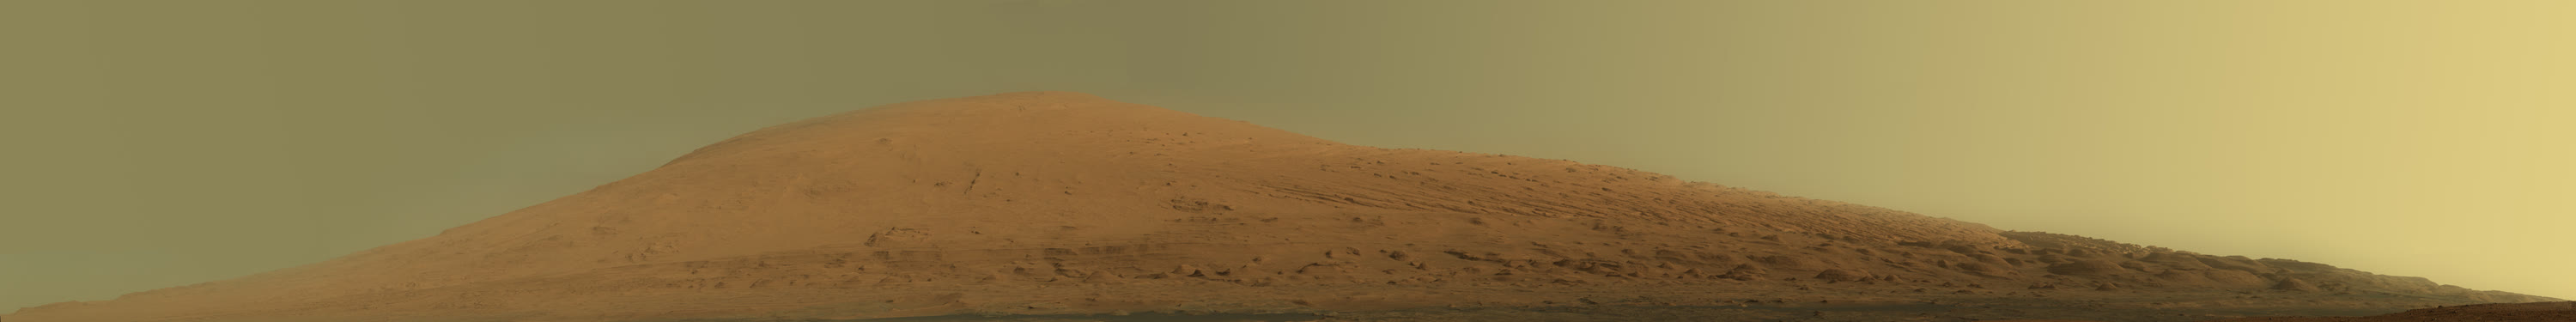
\includegraphics[width=0.96\linewidth]{images/book2/g10-nasa-mars-mount-sharp.jpg}

{\small Mount Sharp, in de Galekrater op Mars, gefotografeerd door de rover
Curiosity in 2012, in de kleuren die zijn camera vastlegde. De onderste lagen
werden miljarden jaren geleden in water afgezet. Beeld: NASA/JPL-Caltech/MSSS
(publiek domein).}
\end{omfigure}

\section{De bewoonbare zone}

\begin{definition}[Bewoonbare zone]\label{def:g10:habitable-planet:habitable-zone}
De \emph{bewoonbare zone}\index{bewoonbare zone} van een ster is het gebied
van afstanden tot de ster waarop een rotsplaneet met genoeg water en een
atmosfeer zoals die van de Aarde vloeibaar water aan haar oppervlak zou kunnen
houden. De binnenrand ligt waar de planeet haar water door de hitte zou
verliezen; de buitenrand waar zelfs een sterk broeikaseffect haar niet meer
zou kunnen behoeden voor bevriezing.
\end{definition}

\begin{proposition}[De bewoonbare zone van de Zon]\label{prop:g10:habitable-planet:hz-sun}
% ledger: kopparapu:hz-sun, planet:Mercury.dist, planet:Venus.dist, planet:Mars.dist
Gedetailleerde modellen van planeetatmosferen plaatsen de \omterm{def:g10:habitable-planet:habitable-zone}{bewoonbare zone} van
de Zon tussen \qty{0.99}{au} en \qty{1.70}{au}. De Aarde (\qty{1}{au}) ligt net
binnen de binnenrand; Mars (\qty{1.52}{au}) ligt erin; Venus
(\qty{0.72}{au}) ligt ruim binnen de binnenrand.
\end{proposition}

\begin{proposition}[Bewoonbare zones van andere sterren]\label{prop:g10:habitable-planet:hz-scaling}
Rond een ster met lichtkracht $L$ ontvangt een planeet dezelfde
bestralingssterkte als op een afstand $d_\odot$ van de Zon wanneer ze ligt op
\[
  d = d_\odot \sqrt{L/L_\odot}.
\]
De randen van de \omterm{def:g10:habitable-planet:habitable-zone}{bewoonbare zone} verschuiven in eerste benadering evenredig mee
(de kleur van het sterlicht speelt ook een kleine rol).
\end{proposition}

\begin{proof}
Gelijke bestralingssterkte betekent $L/(4\pi d^2) = L_\odot/(4\pi d_\odot^2)$, dus
$d^2 = d_\odot^2\,L/L_\odot$.
\end{proof}

\begin{omfigure}
\begin{tikzpicture}[font=\small]
  % top: the Sun, 0-2 au over 12 cm (6 cm per au)
  \fill[omProp!30] (0.99*6,0) rectangle (1.70*6,0.5);
  \draw[black!70] (0,0.25) -- (12.3,0.25);
  \foreach \x in {0,0.5,...,2} \draw (\x*6,0.15) -- (\x*6,0.35) node[pos=0, below=1pt, font=\footnotesize] {\x};
  \shade[ball color=yellow!70!orange] (0,0.25) circle (0.22);
  \foreach \n/\d in {Mercurius/0.387, Venus/0.723, Aarde/1.0, Mars/1.524} {
    \fill[omThm!85!black] (\d*6,0.25) circle (2.2pt);
    \node[anchor=south, font=\footnotesize] at (\d*6,0.55) {\n};
  }
  \node[anchor=west, font=\footnotesize] at (12.4,0.25) {au};
  \node[anchor=north, font=\footnotesize] at (8.07,-0.25) {bewoonbare zone, 0.99--1.70 au};
  \node[anchor=east, font=\footnotesize] at (-0.3,0.25) {Zon};
  % bottom: Proxima Centauri, 0-0.1 au over 12 cm (120 cm per au)
  \begin{scope}[yshift=-2.2cm]
  \fill[omProp!30] (0.0385*120,0) rectangle (0.0661*120,0.5);
  \draw[black!70] (0,0.25) -- (12.3,0.25);
  \foreach \x/\l in {0/0, 0.025/0.025, 0.05/0.05, 0.075/0.075, 0.1/0.1} \draw (\x*120,0.15) -- (\x*120,0.35) node[pos=0, below=1pt, font=\footnotesize] {\l};
  \shade[ball color=red!70!orange] (0,0.25) circle (0.14);
  \fill[omThm!85!black] (0.0485*120,0.25) circle (2.2pt);
  \node[anchor=south, font=\footnotesize] at (0.0485*120,0.55) {Proxima b};
  \node[anchor=west, font=\footnotesize] at (12.4,0.25) {au};
  \node[anchor=north, font=\footnotesize] at (6.28,-0.25) {bewoonbare zone, 0.038--0.066 au};
  \node[anchor=east, align=right, font=\footnotesize] at (-0.3,0.25) {Proxima\\Centauri};
  \end{scope}
\end{tikzpicture}

{\small Boven: de \omterm{def:g10:habitable-planet:habitable-zone}{bewoonbare zone} van de Zon en de vier rotsplaneten. Onder:
de \omterm{def:g10:habitable-planet:habitable-zone}{bewoonbare zone} van de zwakke rode ster Proxima Centauri, berekend door die
van de Zon te schalen met de vierkantswortel van de lichtkracht van de ster, en
haar planeet Proxima~b. Let op de andere schaal: de hele onderste strook is
\qty{0.1}{au} lang.}
\end{omfigure}

\section{Planeten van andere sterren}

\begin{definition}[Exoplaneet]\label{def:g10:habitable-planet:exoplanet}
Een \emph{exoplaneet}\index{exoplaneet} is een planeet die om een andere ster
dan de Zon draait.
\end{definition}

Exoplaneten zijn veel te zwak en staan te dicht bij hun ster om rechtstreeks
gezien te worden, op een paar reuzen na. De meeste worden onrechtstreeks
gevonden: ofwel trekt de planeet één keer per omloop vóór haar ster langs en
maakt die heel lichtjes zwakker, ofwel doet haar aantrekking de ster naar ons
toe en van ons af wiebelen, waardoor de kleur van het sterlicht heen en weer
verschuift. De tweede methode geeft alleen een \emph{minimale} massa voor de
planeet, omdat de helling van de baan niet bekend is. Deze methoden komen aan
bod in het boek voor bachelorjaar~3.

\begin{dated}{2026}
% ledger: nea:count-2026
Op 15 oktober 2026 telde het NASA Exoplanet Archive 6\,451 bevestigde
exoplaneten.
\end{dated}

\begin{example}[Proxima b]\label{ex:g10:habitable-planet:proxima}
% ledger: nea:proxima-b (flux and habitable zone computed in figdata/grade-10/planet_temperatures.py)
De ster die het dichtst bij de Zon staat, Proxima Centauri, op \qty{1.30}{\parsec}, is een
kleine rode ster met een lichtkracht van maar ongeveer $0.0015$ keer die van
de Zon. In 2016 werd een planeet ontdekt die er elke 11.2 dagen omheen draait,
op \qty{0.0485}{au}, met minstens 1.06 keer de massa van de Aarde. Op die
afstand ontvangt ze ongeveer 0.64 keer de bestralingssterkte die de Aarde
ontvangt, en ligt ze binnen de \omterm{def:g10:habitable-planet:habitable-zone}{bewoonbare zone} van haar ster. Of ze een
atmosfeer heeft, of water, is niet bekend.
\end{example}

\begin{remark}[Bewoonbaar is niet bewoond]\label{rem:g10:habitable-planet:inhabited}
De \omterm{def:g10:habitable-planet:habitable-zone}{bewoonbare zone} zegt alleen iets over afstand en licht. Een planeet erin
kan geen water hebben, geen atmosfeer, of de verkeerde --- Mars ligt in de
zone van de Zon en heeft vandaag geen vloeibaar water aan zijn oppervlak. De
Aarde is bewoonbaar omdat verschillende voorwaarden tegelijk vervuld zijn: de
juiste afstand, een massa die groot genoeg is om een atmosfeer vast te houden,
veel water, en een broeikaseffect dat niet te zwak en niet te sterk is.
\end{remark}

\section{Oefeningen}

\begin{exercise}[$\star$]\label{exo:g10:habitable-planet:1}
Definieer de \omterm{def:g10:habitable-planet:equilibrium-temperature}{evenwichtstemperatuur} van een planeet. Waarom is de gemiddelde
oppervlaktetemperatuur van de Aarde hoger dan haar \omterm{def:g10:habitable-planet:equilibrium-temperature}{evenwichtstemperatuur}?
\end{exercise}

\begin{exercise}[$\star$]\label{exo:g10:habitable-planet:2}
Noem met behulp van het staafdiagram van evenwichts- en gemeten temperaturen
het hemellichaam waarvan het oppervlak het sterkst door zijn atmosfeer wordt
opgewarmd, en schat met hoeveel kelvin.
\end{exercise}

\begin{exercise}[$\star$]\label{exo:g10:habitable-planet:3}
Mars draait op \qty{1.52}{au} van de Zon. Bereken met de omgekeerd-kwadratenwet
en $S_0 = \qty{1361}{W/m^2}$ de bestralingssterkte van de Zon bij Mars.
\end{exercise}

\begin{exercise}[$\star$]\label{exo:g10:habitable-planet:4}
Geef met behulp van het fasediagram van water de toestand van water bij
\qty{1}{bar} en \qty{330}{K}; bij \qty{0.001}{bar} en \qty{250}{K}; bij
\qty{100}{bar} en \qty{700}{K}.
\end{exercise}

\begin{exercise}[$\star$]\label{exo:g10:habitable-planet:5}
Wat is een \omterm{def:g10:habitable-planet:exoplanet}{exoplaneet}? Beschrijf in telkens één zin de twee belangrijkste
manieren waarop exoplaneten worden opgespoord.
\end{exercise}

\begin{exercise}[$\star\star$]\label{exo:g10:habitable-planet:6}
Bereken de \omterm{def:g10:habitable-planet:equilibrium-temperature}{evenwichtstemperatuur} van de Aarde met $S_0 = \qty{1361}{W/m^2}$
en $A = 0.294$, en daarna met $A = 0$. Reken beide om naar graden Celsius.
\end{exercise}

\begin{exercise}[$\star\star$]\label{exo:g10:habitable-planet:7}
Een ster is vier keer zo lichtsterk als de Zon. Tussen welke afstanden ligt
haar \omterm{def:g10:habitable-planet:habitable-zone}{bewoonbare zone}? Zou de Aarde, op \qty{1}{au} van deze ster geplaatst,
erbinnen liggen?
\end{exercise}

\begin{exercise}[$\star\star$]\label{exo:g10:habitable-planet:8}
Venus draait op \qty{0.723}{au}. Bereken de bestralingssterkte die ze ontvangt,
en daarna haar \omterm{def:g10:habitable-planet:equilibrium-temperature}{evenwichtstemperatuur} met haar bondalbedo van 0.77. Vergelijk met
haar oppervlaktetemperatuur van \qty{737}{K} en verklaar het verschil.
\end{exercise}

\begin{exercise}[$\star\star$]\label{exo:g10:habitable-planet:9}
Op Mars is de gemiddelde druk aan het oppervlak \qty{6.36}{mbar}, net boven het
tripelpunt van water, en water kookt er bij ongeveer \qty{0.5}{\degreeCelsius}.
Leg uit waarom vloeibaar water vandaag niet kan blijven bestaan aan het oppervlak
van Mars, zelfs niet op een zomermiddag waarop de grond \qty{10}{\degreeCelsius} bereikt.
\end{exercise}

\begin{exercise}[$\star\star$]\label{exo:g10:habitable-planet:10}
De ontsnappingssnelheid is \qty{2.4}{km/s} op de Maan en \qty{11.2}{km/s} op
de Aarde. Bereken hun verhouding. Leg uit waarom de Aarde een atmosfeer heeft
behouden en de Maan niet.
\end{exercise}

\begin{exercise}[$\star\star$]\label{exo:g10:habitable-planet:11}
Stel dat de Aarde met ijs bedekt was en haar bondalbedo tot 0.50 steeg.
Bereken haar nieuwe \omterm{def:g10:habitable-planet:equilibrium-temperature}{evenwichtstemperatuur}. Leg uit waarom zo'n toestand, eenmaal
bereikt, de neiging zou hebben te blijven bestaan.
\end{exercise}

\begin{exercise}[$\star\star\star$]\label{exo:g10:habitable-planet:12}
Laat zien dat $T_{\mathrm{eq}} = \qty{278.3}{K} \times (1-A)^{1/4}/\sqrt{d}$, met
$d$ in astronomische eenheden, volgt uit de formule van het hoofdstuk. Met welke
factor verandert de \omterm{def:g10:habitable-planet:equilibrium-temperature}{evenwichtstemperatuur} als de afstand met vier wordt
vermenigvuldigd?
\end{exercise}

\begin{exercise}[$\star\star\star$]\label{exo:g10:habitable-planet:13}
Op welke afstand van de Zon zou een planeet met albedo 0.294 een
\omterm{def:g10:habitable-planet:equilibrium-temperature}{evenwichtstemperatuur} van \qty{273}{K} hebben? Vergelijk met de binnenrand van
de \omterm{def:g10:habitable-planet:habitable-zone}{bewoonbare zone}, en leg uit waarom die twee verschillen.
\end{exercise}

\begin{exercise}[$\star\star\star$]\label{exo:g10:habitable-planet:14}
Op een planeet met een druk aan het oppervlak van \qty{1000}{Pa} kookt water bij
ongeveer \qty{7}{\degreeCelsius}. Tussen welke temperaturen kan water daar
vloeibaar zijn? Wat zou er met een meer op die planeet gebeuren op een dag van
\qty{15}{\degreeCelsius}?
\end{exercise}

\begin{exercise}[$\star\star\star$]\label{exo:g10:habitable-planet:15}
Een planeet draait op \qty{1.2}{au} van een ster die half zo lichtsterk is als
de Zon. Bereken de randen van de \omterm{def:g10:habitable-planet:habitable-zone}{bewoonbare zone} van de ster en zeg of de planeet
erbinnen ligt. Hoe zeker kun je van het antwoord zijn?
\end{exercise}

\section{Probleem: kan Proxima b een oceaan hebben?}

\begin{problem}[{Weekendprobleem --- van het licht van een zwakke rode ster tot
de temperatuur van haar dichtstbijzijnde planeet}]
\label{pb:g10:habitable-planet:1}
% ledger: nea:proxima-b, kopparapu:hz-sun, earth:TSI, earth:albedo, planet:Earth.vesc, nasa:bond-albedos (all results computed in figdata/grade-10/planet_temperatures.py or from the rounded data below)
Een leerling leest het gegevensblad van de planeet Proxima~b. Haar ster heeft
een lichtkracht $L = 0.00151\,L_\odot$; de planeet draait op $d = \qty{0.0485}{au}$
in 11.18 dagen om de ster en heeft minstens 1.055 keer de massa van de Aarde.
Gebruik $S_0 = \qty{1361}{W/m^2}$, $\sigma = \qty{5.67e-8}{W.m^{-2}.K^{-4}}$, de
\omterm{def:g10:habitable-planet:habitable-zone}{bewoonbare zone} van de Zon \qtyrange{0.99}{1.70}{au}, en de
ontsnappingssnelheid van de Aarde \qty{11.2}{km/s}.

\medskip
\noindent\textbf{Deel I --- Het licht van de ster.}
\begin{enumerate}
  \item Bereken de bestralingssterkte bij de planeet als deel van die bij de
        Aarde, $L/d^2$ (met $L$ in zonnelichtkrachten en $d$ in au).
  \item Druk ze uit in \unit{W/m^2}.
  \item Vergelijk ze met de bestralingssterkte bij Venus (\qty{2601}{W/m^2}) en
        bij Mars (\qty{586}{W/m^2}).
  \item Hoeveel jaren van de planeet passen er in één aardjaar?
\end{enumerate}

\medskip
\noindent\textbf{Deel II --- Temperaturen zonder atmosfeer.}
\begin{enumerate}[resume]
  \item Bereken de \omterm{def:g10:habitable-planet:equilibrium-temperature}{evenwichtstemperatuur} van een volkomen donkere planeet
        ($A = 0$) bij die bestralingssterkte.
  \item Bereken ze voor een planeet die even helder is als Venus ($A = 0.77$).
  \item Welke van deze twee temperaturen ligt boven het vriespunt van water?
        Wat laten de twee resultaten zien over de rol van wolken en
        ijs?
\end{enumerate}

\medskip
\noindent\textbf{Deel III --- De bewoonbare zone.}
\begin{enumerate}[resume]
  \item Bereken $\sqrt{L/L_\odot}$.
  \item Bereken de binnenrand van de \omterm{def:g10:habitable-planet:habitable-zone}{bewoonbare zone} van de ster.
  \item Bereken de buitenrand.
  \item Ligt Proxima~b in de \omterm{def:g10:habitable-planet:habitable-zone}{bewoonbare zone}?
  \item Op welke afstand van de Zon zou een planeet dezelfde
        bestralingssterkte ontvangen als Proxima~b? Waar zou dat in de
        \omterm{def:g10:habitable-planet:habitable-zone}{bewoonbare zone} van de Zon liggen?
\end{enumerate}

\medskip
\noindent\textbf{Deel IV --- Een atmosfeer en water?}
\begin{enumerate}[resume]
  \item Als de planeet de gemiddelde dichtheid van de Aarde had, zou haar straal
        $1.055^{1/3}$ keer die van de Aarde zijn. Bereken deze factor.
  \item De ontsnappingssnelheid is evenredig met $\sqrt{M/R}$. Schat de
        ontsnappingssnelheid van de planeet. Zou ze een atmosfeer kunnen
        vasthouden?
  \item Waarom is de massa alleen als minimum bekend?
  \item Wat is volgens het fasediagram de laagste druk aan het oppervlak
        waarbij vloeibaar water nog mogelijk is?
  \item Bereken de \omterm{def:g10:habitable-planet:equilibrium-temperature}{evenwichtstemperatuur} van Proxima~b met het albedo van de
        Aarde, 0.294.
  \item Met hoeveel kelvin zou haar broeikaseffect haar dan moeten opwarmen om
        haar oppervlak op de gemiddelde temperatuur van de Aarde,
        \qty{288}{K}, te brengen?
\end{enumerate}
\end{problem}
